\section{Homogena ekvationssystem (Avs 5.5)}
Ett ekvationssystem där högerledet är $\bm{0}$ kallas homogent.
Vi tittar på ekvationssystem som ser ut typ $\begin{cases}
    x+y+=0\\
    2x+3y+z=0\\
    x-y+2z=0
\end{cases}$
En lösning ges av x=y=z=0. 
Men vi vill hitta alla lösningar.

\paragraph{Proposition 5.31} Ekvationssytemet $A\bm{x}=\bm{0}$ har alltid lösningen $\bm{x}=\bm{0}$.
Det finns fler lösningar om och endast om totalmatrisen är har fria kolumner efter reducering.

\paragraph{Proposition 5.33} Om $\bm{x}_{p}$ löser $A\bm{x}=\bm{0}$ då ges alla lösningar till $A\bm{x}=\bm{0}$ av $\bm{x}=\bm{x}_{p}$
där $\bm{x}_{n}$ är en lösning till $A\bm{x}=\bm{0}$.
\subparagraph{Bevis} Om $\bm{x}_{p}$ och $\bm{x}$ löser $A\bm{x}=\bm{b}$ då gäller att $A(\bm{x}-\bm{x}_{p})=A\bm{x}-A\bm{x}_{p}=\bm{b}-\bm{b}=\bm{0}$
och alltså löser $\bm{x}-\bm{x}_{p}$ ekvationen $A\bm{x}=\bm{0}$

\paragraph{Ex} Systemet $\begin{cases}
    x+y+z=2\\x+2y+2z=3\\2x+3y+3z=5
\end{cases}$ har en lösning $\begin{cases}
    x=1\\y=1\\z=0
\end{cases}$.
Hitta alla!
\subparagraph{Lösning} Engligt Prop 5.33 kan vi lösa det homogena systemet:
$\begin{cases}
    x+y+z=0\\
    x+2y+2z=0\\
    2x+2y+3z=0
\end{cases}$
Totalmatrisen: $\begin{pmatrix}
    1&1&1&0\\
    1&2&2&0\\
    2&3&3&0
\end{pmatrix}
\thicksim
\begin{pmatrix}
    1&1&1&0\\
    0&1&1&0\\
    0&1&1&0
\end{pmatrix}
\thicksim
\begin{pmatrix}
    1&1&1&0\\
    0&1&1&0\\
    0&0&0&0
\end{pmatrix}$\\
Vi sätter $z=t$.
\begin{equation*}
    \begin{cases}
        x+y+z=0\\
        y+z=0
    \end{cases}
    \Rightarrow
    \begin{cases}
        x=0\\
        y=-t\\
        z=t
    \end{cases}
\end{equation*}
Detta är lösningarna till det homogena systemet.
Samtliga lösningar till det ursprungliga systemet ges av $\begin{cases}
    x=1\\
    y=-t\\
    z=0+t
\end{cases}
\Rightarrow
\begin{pmatrix}
    x\\y\\z
\end{pmatrix}=
\begin{pmatrix}
    1\\1\\0
\end{pmatrix}+t\begin{pmatrix}
    0\\-1\\1
\end{pmatrix}$


\section{Överbestämda ekvationssystem (Avs 5.6)}
\begin{wrapfigure}{r}{0.55\textwidth}
    \vspace{-13pt}
    \centering
    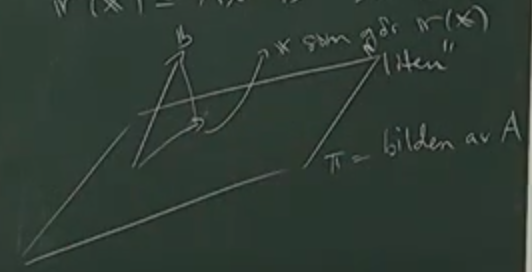
\includegraphics[scale=0.44]{imgs/img01.png}
    \vspace{-20pt}
\end{wrapfigure}
Vi tittar nu på ekvationssytem med fler ekvationer än variabler.
Vi förväntar oss i allmänhet att dessa saknar lösningar.
Vi vill alltså lösa $A\bm{x}=\bm{b}$ men det kanske inte går.
Då vill vi istället göra $\bm{r}(\bm{x})=A\bm{x}-\bm{b}$ så litet som möjligt.

\paragraph{Proposition 5.36} Lösningen till $A^{t}A\bm{x}=A^{t}\bm{b}$ gör att $\bm{r}=A\bm{x}-\bm{b}$ är "så liten som möjligt".
"minsta kvadratmetoden".
Observera att om $A$ är en $m\times n$-matris då är $A^{t}$ en $n\times m$-matris och $A^{t}A$ är en $n\times n$-matris.\\
Det finns en unik lösning till $A^{t}A\bm{x}=A^{t}\bm{b}\Leftrightarrow det(A^{t}A)\neq 0$.

\clearpage

\paragraph{Ex} Hitta den linje $y=kx+m$ som närmast passar punkterna $(1,1)$, $(1,2)$, $(4,5)$.
\subparagraph{Lösning}
\begin{wrapfigure}{r}{0.45\textwidth}
    \vspace{-25pt}
    \centering
    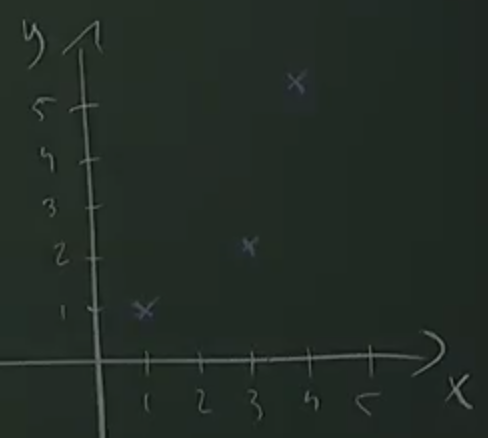
\includegraphics[scale=0.42]{imgs/img02.png}
    \vspace{-50pt}
\end{wrapfigure}
Vi vill att $\begin{cases}k+m=1\\3k+m=2\\4k+m=5\end{cases}$
\begin{equation*}
    A=\begin{pmatrix}
        1&1\\
        3&1\\
        4&1
    \end{pmatrix},
    \bm{b}=\begin{pmatrix}
        1\\2\\5
    \end{pmatrix}
    \Leftrightarrow
    A\begin{pmatrix}
        k\\m
    \end{pmatrix}=\bm{b}
\end{equation*}
Men $A\begin{pmatrix}k\\m\end{pmatrix}$ saknar lösningar så vi\\ tittar istället på $A^{t}A\begin{pmatrix}k\\m\end{pmatrix}=A^{t}\bm{b}$.
\begin{enumerate}
    \item[] 
        $A^{t}A=\begin{pmatrix}
            1&3&4\\
            1&1&1
        \end{pmatrix}
        \begin{pmatrix}
            1&1\\
            3&1\\
            4&1
        \end{pmatrix}
        =
        \begin{pmatrix}
            16&8\\
            8&3
        \end{pmatrix}$
    \item[] 
        $A^{t}\bm{b}=
        \begin{pmatrix}
            1&3&4\\
            1&1&1
        \end{pmatrix}
        \begin{pmatrix}
            1\\2\\5
        \end{pmatrix}
        =
        \begin{pmatrix}
            27\\8
        \end{pmatrix}$ 
\end{enumerate}
\begin{center}
    $\text{Vi löser }A^{t}A
    \begin{pmatrix}
        k\\
        m
    \end{pmatrix}=
    \begin{pmatrix}
        27\\
        8
    \end{pmatrix}
    \Leftrightarrow
    \begin{pmatrix}
        26&8&27\\
        8&3&8
    \end{pmatrix}
    \thicksim
    \begin{pmatrix}
        26\cdot 4&8\cdot 4&27\cdot 4\\
        8\cdot 13&3\cdot 13&8\cdot 13
    \end{pmatrix}$\\
    $\thicksim
    \begin{pmatrix}
        26&8&27\\
        0&7&-4
    \end{pmatrix}
    \Leftrightarrow
    \begin{cases}
        26k+8m-=27\\
        7m=-4
    \end{cases}
    \Leftrightarrow
    \begin{cases}
        k=\frac{27+\frac{8\cdot4}{7}}{26}\\
        m=-\frac{4}{7}
    \end{cases}
    $
\end{center}

\chapter{Determinanter}
För $2\times 2$- och $3\times 3$-matriser har vi sett att
\begin{enumerate}
    \item $det(I_{n})=1$
    \item determinanten är linjär i varje kolumn:
        \begin{equation*}
            det(\bm{a}_{1}\text{ }\ldots\text{ }b\bm{a}_{k}+c\widehat{\bm{a}}_{k}\text{ }\ldots\text{ }\bm{a}_{n}=
            bdet(\bm{a}_{1}\text{ }\ldots\text{ }\bm{a}_{k}\text{ }\ldots\text{ }\bm{a}_{n}+
            cdet(\bm{a}_{1}\text{ }\ldots\text{ }\widehat{\bm{a}}_{k}\text{ }\ldots\text{ }\bm{a}_{n})
        \end{equation*}
    \item om två kolumner är likadana då är determinanten noll
\end{enumerate}

\paragraph{Definition} För $n\times n$-matriser är determinanten den unika funktion ådan att:
\begin{enumerate}
    \item $det(I_{n})$
    \item determinanten är linjär i varje kolumn
    \item om två kolumner är likadana så är determinanten noll
\end{enumerate}

\paragraph{Proposition 6.4} Antag att vi gör en elementär radoperation på $1\times 1$-matris $A$ 
och får matrisen $B$. Då gäller:
\begin{enumerate}[label=\alph*]
    \item Om vi bytt plats på två rader då är $det(B)=-det(A)$
    \item Om vi har multiplicerat en rad med ett tal $c$ då är $det(B)=cdet(A)$
    \item Om vi har adderat en multipel av en rad på en annan då är $det(B)=det(A)$
\end{enumerate}

\paragraph{Sats 6.5} Antag att $A$ är över- eller undertriangulär (dvs bara nollor ovan/under diagonalen).
Då är $det(A)=a_{11}\text{ }a_{22}\text{ }\ldots\text{ }a_{nn}$

\paragraph{Ex} Beräkna determinanten av $A=\begin{pmatrix}
    1&2&5&0\\
    5&-3&9&6\\
    3&0&19&0\\
    0&0&8&0
\end{pmatrix}$
\subparagraph{Lösning} $det(A)=\begin{vmatrix}
    1&2&5&0\\
    5&-3&9&6\\
    3&0&19&0\\
    0&0&8&0
\end{vmatrix}=
\begin{vmatrix}
    1&2&5&0\\
    0&-13&16&6\\
    0&-6&4&0\\
    0&0&8&0
\end{vmatrix}=
\begin{vmatrix}
    1&2&5&0\\
    0&-13&16&6\\
    0&0&4+\frac{\cdot 16}{6}&-13\\
    0&0&8&0
\end{vmatrix}=
\begin{vmatrix}
    1&2&5&0\\
    0&-13&16&6\\
    0&0&\frac{208}{6}&-13\\
    0&0&0&\frac{6\cdot 8\cdot 13}{208}
\end{vmatrix}=1\cdot (-13)\cdot \frac{208}{6}\cdot \frac{6\cdot 8 \cdot 13}{208}=-8\cdot 13^{2}$

\section{Konstruktion av determinanten (Avs 6.2)}
En bijektiv funktion från $\{1,2,\ldots,n\}$ till $\{1,2,\ldots,n\}$ kallas för en \underline{permutation}.
Till exempel är $\pi$  som ges av $\pi (k)=\varphi$, $\pi (\varphi)=k$, $\pi (i)=i$ för alla $i+k,i\neq\varphi$ en permutation.
En sådan permutation kallas för en \underline{omkastning}.
Varje permutation går att skriva som en serie av omkastningar.
Vi definierar signaturen av en permutation $\pi$ som $\varepsilon (\pi)=(-1)^{k} \text{ }(sgn(\pi))$ där $k$ är antalet omkastningar som $\pi$ går att skriva som.
Signaturen är $-1$ eller 1 (man behöver visa att signaturen är väldefinierad).
\begin{enumerate}
    \item[] Signaturen av omkastning är $-1$.
    \item[] Signaturen av identitetspermutation är 1.
\end{enumerate}

Determinanten av $n\times n$-matrisen $A=\begin{pmatrix}
    a_{11}&a_{12}&\ldots& a_{1n}\\
    a_{21}&a_{22}&\ldots&a_{2n}\\
    \vdots&\vdots&\ddots&\vdots\\
    a_{n1}&a_{n2}&\ldots&a_{nn}
\end{pmatrix}$
ges av 
\begin{equation*}
    det(A)\sum_{\pi\in S_{n}}\varepsilon(\pi)a_{1\pi(1)}a_{2\pi(2)}\ldots a_{n\pi(n)}
\end{equation*}
där $S_{n}$ är mängden av alla permutationer.
